\section{Numerical evidence}\label{sec:exp}

The law is an equality without free constants; each experiment below compares a measured quantity with a number
computed beforehand from the noise law. Details are in \cref{app:exp}.

\begin{table}[t]
\caption{The constants of \cref{thm:two} (exact, to the digits shown) and the proved bounds
$\frac3{K+d+1}<a_1+a_2<\frac3{\max(K,d)+2}$ of \cref{cor:dim}.}
\label{tab:const}
\centering\footnotesize\setlength{\tabcolsep}{3pt}
\begin{tabular}{@{}lcccccc@{}}
\toprule
size & $q_{K,d}$ & $a_1$ & $a_2$ & lower & $a_1+a_2$ & upper\\
\midrule
$2\times2$ & 0.3204 & $-0.4132$ & 1.0958 & 0.6000 & 0.6826 & 0.7500\\
$2\times3$ & 0.3934 & $-0.2041$ & 0.7721 & 0.5000 & 0.5680 & 0.6000\\
$3\times3$ & 0.6869 & $-0.1685$ & 0.6933 & 0.4286 & 0.5249 & 0.6000\\
$4\times4$ & 1.0679 & $-0.0947$ & 0.5226 & 0.3333 & 0.4280 & 0.5000\\
$8\times8$ & 2.6350 & $-0.0249$ & 0.2730 & 0.1765 & 0.2481 & 0.3000\\
$16\times16$ & 5.8149 & $-0.0065$ & 0.1420 & 0.0909 & 0.1355 & 0.1667\\
$64\times64$ & 24.9957 & $-0.0004$ & 0.0369 & 0.0233 & 0.0365 & 0.0455\\
$8\times32$ & 3.3508 & $-0.0023$ & 0.0880 & 0.0732 & 0.0856 & 0.0882\\
$32\times128$ & 14.9400 & $-0.0002$ & 0.0225 & 0.0186 & 0.0223 & 0.0231\\
\bottomrule
\end{tabular}
\end{table}

\begin{figure}[t]
\centering
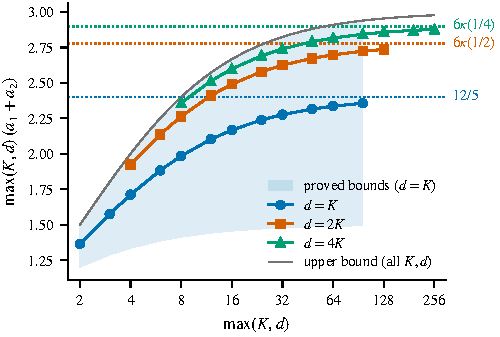
\includegraphics[width=0.92\columnwidth]{fig_constants.pdf}
\caption{The dimension factor of \cref{cor:dim}: $\max(K,d)(a_1+a_2)$ for three aspect ratios (exact values), the
proved bounds for square matrices (band; thin lines for the other ratios), and the proportional limits
$6\kappa(\gamma)$ (dotted).}
\label{fig:const}
\end{figure}

\textbf{Constants.} \cref{tab:const} and \cref{fig:const} give $q_{K,d}$, $a_1$, $a_2$, computed to high precision from the
exact formula for fractional moments of real Wishart matrices. In all $34$ sizes computed, $a_1<0<a_2$, the bounds
of \cref{cor:dim} hold, and $\max(K,d)(a_1+a_2)$ increases to the Marchenko--Pastur limit ($2.357$ at $96\times96$
against $\frac{12}5$).

\begin{figure*}[t]
\centering
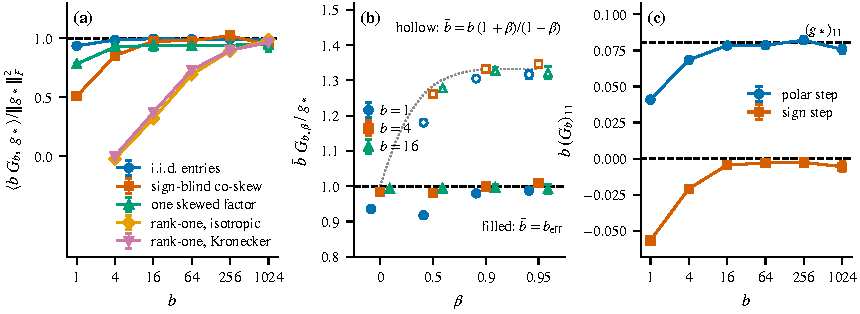
\includegraphics[width=\textwidth]{fig_law.pdf}
\caption{Tests of the first-order law on $2\times3$ matrices (zeros of the mean field, Monte Carlo with standard
errors). (a) $\inner{b\,G_b}{\gs}/\nF{\gs}^2$ for five noise laws; prediction: $1$. (b) Momentum: the zero for the
filtered noise, multiplied by a candidate effective batch size and divided by $\gs$; filled: $\beff$; hollow: the
variance-effective batch size; dotted: the predicted ratio $(1+\beta)^2/(1+\beta+\beta^2)$ of the two. (c) A noise law
whose entries have zero third cumulants: sign descent is unbiased to first order, the orthogonalized step is not.}
\label{fig:law}
\end{figure*}

\textbf{The law across noise laws} (\cref{fig:law}a). We compute the zero $G_b$ of $G\mapsto\E\polar(G+\xi_b)$ for
five laws on $\R^{2\times3}$: independent skewed entries; a ``sign-blind'' law with co-skewness only; one skewed
factor plus symmetric noise; and two rank-one laws $\delta x^\top$, with isotropic and with Kronecker covariance (for
the latter $\gs$ is evaluated from \eqref{eq:gs} by Monte Carlo). The ratio $\inner{bG_b}{\gs}/\nF{\gs}^2$ approaches
$1$ for four of the five laws: $0.990\pm0.003$ (i.i.d., $b\ge64$), $0.986\pm0.017$ (co-skew), $0.986\pm0.011$ and
$0.964\pm0.025$ (rank one, $b=1024$). For the one-factor law it stays at $0.94\pm0.02$ for all $b\ge16$, a deviation
of three standard errors that we cannot explain. Convergence is slow for the rank-one laws ($0.7$ at $b=64$; at
$b=4$ the isotropic one even has the opposite sign); we have no explanation for this either.

\textbf{Momentum} (\cref{fig:law}b). For exponentially filtered noise with $\beta\in\{0,0.5,0.9,0.95\}$ the zero
times $\beff$ is within $2\%$ of $\gs$ for $b\ge4$. Normalizing by the variance-effective batch size instead
gives $1.26$ to $1.35$, the predicted ratio $(1+\beta)^2/(1+\beta+\beta^2)$. The coupled iteration \eqref{eq:muon} on a
quadratic agrees with the zero of the frozen field (\cref{app:exp}).

\textbf{Sign-blind noise} (\cref{fig:law}c). For a law whose entries all have zero third cumulant but
$\E[\zeta_{11}\zeta_{12}^2]\ne0$, the sign step has no first-order offset (measured $b\,G_b$ compatible with $0$ for
$b\ge64$) and the polar step has the offset of \cref{cor:compare}: $0.078$ to $0.082$ measured for $b=16,\dots,256$
and $0.076\pm0.003$ at $b=1024$, against $0.0803$ predicted.

\begin{figure*}[t]
\centering
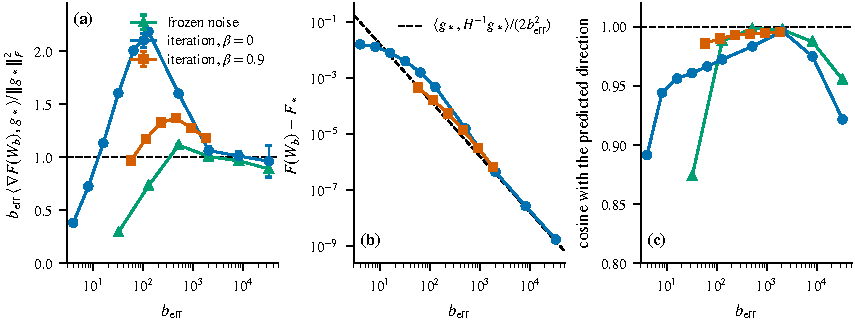
\includegraphics[width=\textwidth]{fig_digits.pdf}
\caption{Real data, no fitted parameter: least squares on \texttt{digits} ($W\in\R^{4\times16}$, $n=1797$,
minibatches with replacement). (a) The stationary gradient along the prediction, scaled by $\beff$; prediction: $1$.
Green: noise frozen at $W_\ast$ (\cref{thm:cf}); blue, red: limit of the iteration \eqref{eq:muon}, whose noise depends
on $W$ (compare \cref{thm:state}, which locates the zero of the mean field for $\beta=0$). (b) Excess loss at the limit against $\inner{\gs}{H^{-1}\gs}/(2\beff^2)$. (c) Cosine between
the measured and the predicted displacement.}
\label{fig:digits}
\end{figure*}

\textbf{A finite-sum problem on real data} (\cref{fig:digits}). We take ridge-regularized least squares on the
\texttt{digits} data set, with $16$ principal components as features and $4$ random projections of the one-hot
labels as targets, so that the covariance of the per-sample gradients is well conditioned. From the $1797$
per-sample gradients at the minimizer we compute $\Sigma$, $K_3$ and $\gs$ (by \eqref{eq:gs}; $\nnuc{\gs}=3.80\pm0.01$),
and compare with the limit of the iteration. The per-sample gradients have rank one and the noise depends on $W$,
so this tests \cref{thm:cf,thm:beff,thm:state} together, away from their idealizations. Three observations.
(i) \emph{The limit is the predicted one at large batch}: the scaled gradient along $\gs$ is $1.06\pm0.04$,
$1.01\pm0.05$, $0.96\pm0.15$ at $b=2048,8192,32768$ (batches larger than the data set, drawn with replacement), the
excess loss is $11$ to $15\%$ above $\inner{\gs}{H^{-1}\gs}/(2b^2)$ over these batch sizes, and the cosine with the
predicted direction reaches $0.997$. (ii) \emph{The approach is slow and not monotone}: the ratio is $0.38$, $0.72$ at
$b=4,8$, then for $16\le b\le512$ the stationary gradient overshoots the prediction, by a factor up to $2.2$ at
$b=128$ ($4.7$ in excess loss), while its direction is already right (cosine $0.97$). With the noise frozen at $W_\ast$
the ratio is $0.29$, $0.73$, $1.11$, $1.006\pm0.012$ at $b=32,128,512,2048$: most of the overshoot is therefore due to
the dependence of the noise on $W$, while a slower, also non-monotone approach remains for frozen noise. We
conjecture that the transient is governed by a second-order term in the dependence on $W$; we have no theory for
it. For reference, $\gs^\top\Sigma^{-1}\gs\approx26$ is the batch size at which the offset equals one standard deviation
of the noise; the transient lasts some $20$ to $80$ times longer. (iii) \emph{Momentum}: with $\beta=0.9$ the same
quantities are closer to the prediction at equal $\beff$ (ratio $0.97$ to $1.37$ for the gradient, $0.93$ to $1.86$ for
the excess loss), but the two curves do not collapse onto one function of $\beff$ in the transient regime. The
first-order law is thus an asymptotic statement whose range of validity, on this problem, is
$\beff\gtrsim2\cdot10^3$; below, it gives the direction and the order of magnitude.
